% Methodology / pipeline diagram. Compile from this folder:
%   pdflatex -interaction=nonstopmode -halt-on-error -output-directory=../Figures fig_pipeline.tex
% Include in main.tex:
%   
\includegraphics[width=\linewidth]{Figures/fig_pipeline}
\documentclass[tikz,border=7pt]{standalone}
\usepackage[scaled=0.95]{helvet}
\renewcommand{\familydefault}{\sfdefault}
\usepackage{xcolor}
\usetikzlibrary{arrows.meta,calc,fit,backgrounds}

\definecolor{ink}{HTML}{1F2933}
\definecolor{muted}{HTML}{5B6776}
\definecolor{line}{HTML}{9AA7B5}
\definecolor{panel}{HTML}{F7F9FC}
\definecolor{bluefill}{HTML}{E8EEF5}
\definecolor{greenfill}{HTML}{EAF4EC}
\definecolor{amberfill}{HTML}{FFF4E3}
\definecolor{accent}{HTML}{255E88}

\begin{document}
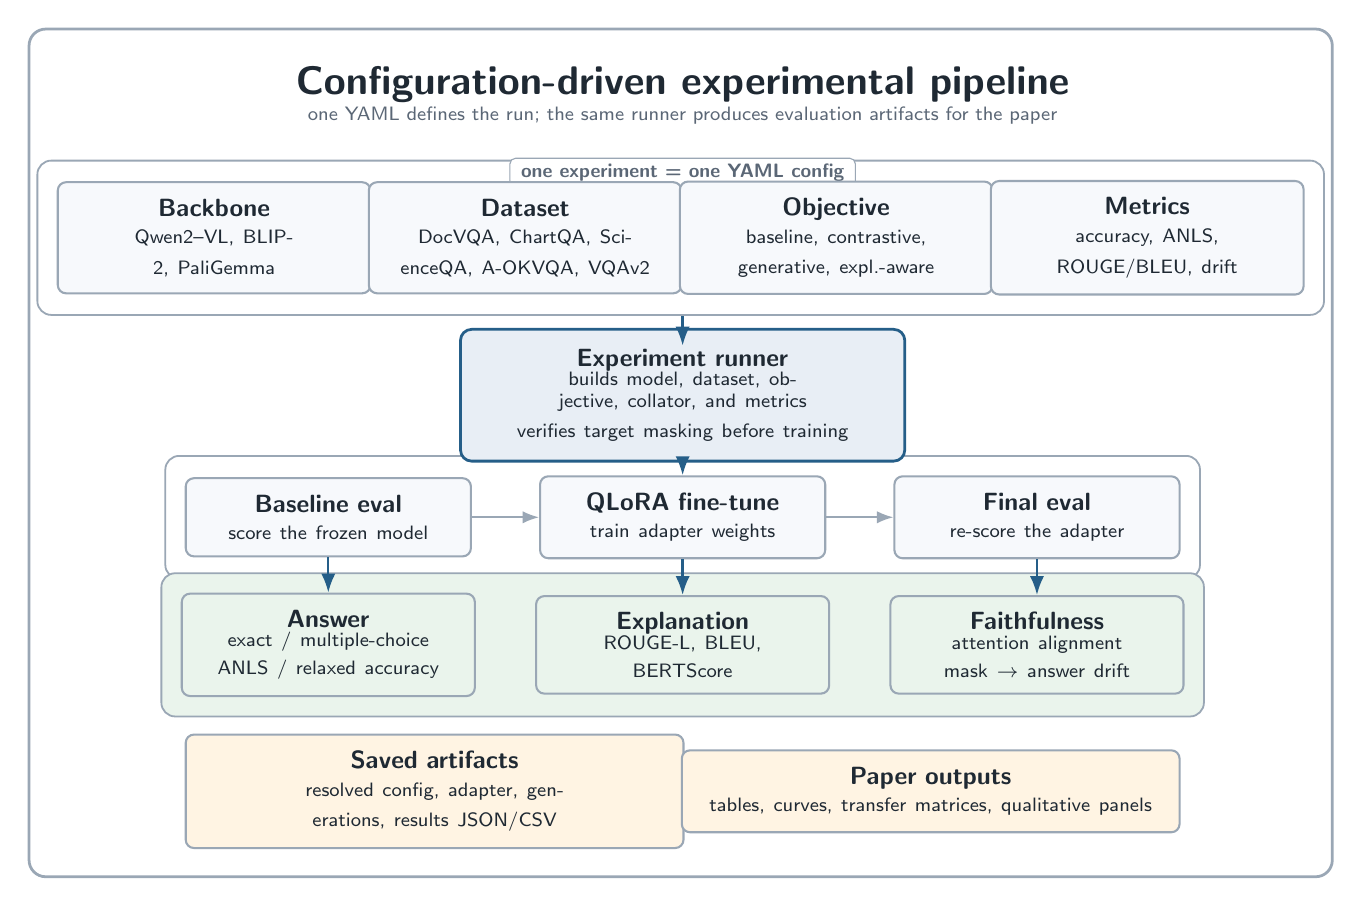
\begin{tikzpicture}[
  font=\sffamily\small,
  >=Latex,
  arrow/.style={->,line width=0.85pt,draw=accent},
  guide/.style={->,line width=0.65pt,draw=line},
  card/.style={draw=line,fill=panel,rounded corners=3pt,line width=0.75pt,
               inner sep=6pt,align=center,text=ink},
  main/.style={draw=accent,fill=bluefill,rounded corners=4pt,line width=1.0pt,
               inner sep=7pt,align=center,text=ink},
  metric/.style={draw=line,fill=greenfill,rounded corners=3pt,line width=0.75pt,
                 inner sep=6pt,align=center,text=ink},
  artifact/.style={draw=line,fill=amberfill,rounded corners=3pt,line width=0.75pt,
                   inner sep=6pt,align=center,text=ink},
  chip/.style={draw=line,fill=white,rounded corners=2pt,inner xsep=4pt,inner ysep=2pt,
               font=\scriptsize\bfseries,text=muted},
  title/.style={font=\sffamily\Large\bfseries,text=ink},
  subtitle/.style={font=\sffamily\scriptsize,text=muted}
]

% Title
\node[title] (title) at (8.5,9.20) {Configuration-driven experimental pipeline};
\node[subtitle] at (8.5,8.80)
  {one YAML defines the run; the same runner produces evaluation artifacts for the paper};

% Config row
\node[chip] (cfglabel) at (8.5,8.08) {one experiment = one YAML config};
\node[card,text width=3.55cm,minimum height=0.95cm] (c1) at (2.55,7.25)
  {\textbf{Backbone}\\[-1pt]\scriptsize Qwen2--VL, BLIP-2, PaliGemma};
\node[card,text width=3.55cm,minimum height=0.95cm] (c2) at (6.50,7.25)
  {\textbf{Dataset}\\[-1pt]\scriptsize DocVQA, ChartQA, ScienceQA, A-OKVQA, VQAv2};
\node[card,text width=3.55cm,minimum height=0.95cm] (c3) at (10.45,7.25)
  {\textbf{Objective}\\[-1pt]\scriptsize baseline, contrastive, generative, expl.-aware};
\node[card,text width=3.55cm,minimum height=0.95cm] (c4) at (14.40,7.25)
  {\textbf{Metrics}\\[-1pt]\scriptsize accuracy, ANLS, ROUGE/BLEU, drift};

% Runner
\node[main,text width=5.15cm,minimum height=1.08cm] (runner) at (8.5,5.25)
  {\textbf{Experiment runner}\\[-1pt]
   \scriptsize builds model, dataset, objective, collator, and metrics\\
   \scriptsize verifies target masking before training};

% Run stages
\node[card,text width=3.2cm,minimum height=0.88cm] (s1) at (4.0,3.70)
  {\textbf{Baseline eval}\\[-1pt]\scriptsize score the frozen model};
\node[card,text width=3.2cm,minimum height=0.88cm] (s2) at (8.5,3.70)
  {\textbf{QLoRA fine-tune}\\[-1pt]\scriptsize train adapter weights};
\node[card,text width=3.2cm,minimum height=0.88cm] (s3) at (13.0,3.70)
  {\textbf{Final eval}\\[-1pt]\scriptsize re-score the adapter};

% Evaluation outputs
\node[metric,text width=3.3cm,minimum height=1.0cm] (m1) at (4.0,2.08)
  {\textbf{Answer}\\[-1pt]\scriptsize exact / multiple-choice\\[-1pt]\scriptsize ANLS / relaxed accuracy};
\node[metric,text width=3.3cm,minimum height=1.0cm] (m2) at (8.5,2.08)
  {\textbf{Explanation}\\[-1pt]\scriptsize ROUGE-L, BLEU,\\[-1pt]\scriptsize BERTScore};
\node[metric,text width=3.3cm,minimum height=1.0cm] (m3) at (13.0,2.08)
  {\textbf{Faithfulness}\\[-1pt]\scriptsize attention alignment\\[-1pt]\scriptsize mask $\rightarrow$ answer drift};

% Artifacts
\node[artifact,text width=5.9cm,minimum height=0.8cm] (a1) at (5.35,0.22)
  {\textbf{Saved artifacts}\\[-1pt]\scriptsize resolved config, adapter, generations, results JSON/CSV};
\node[artifact,text width=5.9cm,minimum height=0.8cm] (a2) at (11.65,0.22)
  {\textbf{Paper outputs}\\[-1pt]\scriptsize tables, curves, transfer matrices, qualitative panels};

% Flow arrows: vertical and evenly spaced
\draw[arrow] (8.5,6.25) -- (8.5,5.88);
\draw[arrow] (runner.south) -- (s2.north);
\draw[guide] (s1.east) -- (s2.west);
\draw[guide] (s2.east) -- (s3.west);
\draw[arrow] (s1.south) -- (m1.north);
\draw[arrow] (s2.south) -- (m2.north);
\draw[arrow] (s3.south) -- (m3.north);

\begin{scope}[on background layer]
  \node[draw=line,fill=white,rounded corners=6pt,line width=1.0pt,
        fit=(title)(cfglabel)(c1)(c4)(runner)(s1)(s3)(m1)(m3)(a1)(a2),
        inner sep=10pt] {};
  \node[draw=line,fill=white,rounded corners=5pt,line width=0.65pt,
        fit=(c1)(c2)(c3)(c4),inner sep=7pt] {};
  \node[draw=line,fill=white,rounded corners=5pt,line width=0.65pt,
        fit=(s1)(s2)(s3),inner sep=7pt] {};
  \node[draw=line,fill=greenfill,rounded corners=5pt,line width=0.65pt,
        fit=(m1)(m2)(m3),inner sep=7pt] {};
\end{scope}

\end{tikzpicture}
\end{document}
